\documentclass[11pt,letterpaper]{article}
\input{glyphtounicode}
\pdfgentounicode=1
\usepackage[utf8]{inputenc}
\usepackage[T1]{fontenc}
\usepackage{lmodern}
\usepackage[spanish,es-noindentfirst,es-tabla]{babel}
\decimalpoint
\usepackage[margin=2.5cm]{geometry}
\usepackage{graphicx}
\usepackage{booktabs}
\usepackage{array}
\usepackage{multirow}
\usepackage{siunitx}
\sisetup{output-decimal-marker={.}, group-digits=false, detect-weight=true, table-number-alignment=center}
\usepackage{amsmath,amssymb}
\usepackage{listings}
\renewcommand{\lstlistingname}{Código}
\usepackage{xcolor}
\usepackage{tikz}
\usetikzlibrary{positioning,arrows.meta,shapes.geometric}
\usepackage{fancyhdr}
\usepackage{titlesec}
\usepackage{caption}
\usepackage[section]{placeins}
\usepackage[hidelinks]{hyperref}
\graphicspath{{figuras/}}
\renewcommand{\topfraction}{0.92}
\renewcommand{\bottomfraction}{0.85}
\renewcommand{\textfraction}{0.06}
\renewcommand{\floatpagefraction}{0.80}
\setcounter{topnumber}{3}
\setcounter{totalnumber}{5}
\captionsetup{font=small,labelfont=bf}

\lstdefinestyle{codigo}{
    language=Python,
    basicstyle=\ttfamily\footnotesize,
    keywordstyle=\color{blue!60!black}\bfseries,
    commentstyle=\color{gray},
    stringstyle=\color{orange!70!black},
    numbers=left,
    numberstyle=\tiny\color{gray},
    frame=single,
    breaklines=true,
    showstringspaces=false,
    tabsize=4,
    backgroundcolor=\color{gray!5},
    extendedchars=true,
    columns=fullflexible,
    keepspaces=true,
    literate={á}{{\'a}}1 {é}{{\'e}}1 {í}{{\'i}}1 {ó}{{\'o}}1 {ú}{{\'u}}1
             {Á}{{\'A}}1 {É}{{\'E}}1 {Í}{{\'I}}1 {Ó}{{\'O}}1 {Ú}{{\'U}}1
             {ñ}{{\~n}}1 {Ñ}{{\~N}}1 {¿}{{?`}}1 {¡}{{!`}}1 {±}{{$\pm$}}1
}
\lstset{style=codigo}

\pagestyle{fancy}
\fancyhf{}
\rhead{Inteligencia Computacional Aplicada}
\cfoot{\thepage}
\renewcommand{\headrulewidth}{0.4pt}
\titleformat{\section}{\normalfont\Large\bfseries}{\thesection.}{0.5em}{}
\titleformat{\subsection}{\normalfont\large\bfseries}{\thesubsection}{0.5em}{}

\newcommand{\nombreEstudiante}{Sergio Santiago Duarte Rojas}
\newcommand{\codigoEstudiante}{20261595002}
\newcommand{\nombreDocente}{Cesar Andrey Perdomo Charry}
\newcommand{\nombreAsignatura}{Inteligencia Computacional Aplicada}

% Diagramas de arquitectura
\definecolor{cEntrada}{RGB}{230,230,230}
\definecolor{cConv}{RGB}{204,224,240}
\definecolor{cPool}{RGB}{255,228,204}
\definecolor{cDensa}{RGB}{212,236,222}
\definecolor{cReg}{RGB}{236,220,240}
\tikzset{
    capa/.style={draw=black!60, rounded corners=2pt, minimum height=1.05cm, text width=1.95cm, align=center, font=\footnotesize, inner sep=2pt},
    tensor/.style={font=\scriptsize, text=black!70},
    flecha/.style={-{Latex[length=1.6mm]}, black!70},
}
\definecolor{cDifuso}{RGB}{255,240,200}

\input{cifras}
\hypersetup{pdftitle={Actividad 4. Taller propuesto de lógica difusa}, pdfauthor={Sergio Santiago Duarte Rojas}}
\lhead{Actividad 4, taller propuesto}

\begin{document}

\begin{titlepage}
    \centering
    \vspace*{2cm}
    {\LARGE \bfseries Actividad 4. Taller propuesto\\[4pt] Reglas difusas extraídas de los datos y ajuste de un sistema difuso\par}
    \vspace{0.5cm}
    {\large Informe de ejecución\par}
    \vspace{2cm}
    \begin{tabular}{ll}
        \textbf{Asignatura:} & \nombreAsignatura \\
        \textbf{Docente:}    & \nombreDocente \\
        \textbf{Estudiante:} & \nombreEstudiante \\
        \textbf{Código:}     & \codigoEstudiante \\
        \textbf{Fecha:}      & \today \\
    \end{tabular}
    \vfill
    Universidad Distrital Francisco José de Caldas
\end{titlepage}

\tableofcontents
\newpage

\section{Introducción}

El cuaderno resuelto de la clase construye conjuntos difusos, un sistema Mamdani, un Sugeno de orden cero, un clasificador con reglas extraídas de Iris y un agrupamiento con Fuzzy C-Means. El taller propuesto aplica lo mismo a Wine en seis tareas, que la diapositiva del bloque 10 presenta así. Primero se eligen cuatro características solo con el entrenamiento y se programa la función sigmoidal \texttt{sigmf}. Después se calcula la fuerza de las reglas con mínimo y con producto, y se obtienen la matriz de confusión y el par más confundido. Por último se comparan etiquetas, reglas, exactitud y un árbol de decisión, y se agrupa con FCM exportando los datos para MATLAB. El enunciado del aula agrega el ejemplo de MathWorks para ajustar un sistema difuso con \texttt{tunefis}.

El aula adjunta el taller como live script de MATLAB y el cuaderno resuelto de la clase en Python. Este informe resuelve las tareas de la diapositiva en un cuaderno de Python armado sobre el resuelto, cuyas funciones se usan sin cambios, con un bloque \texttt{TODO} por tarea. Las dos piezas que dependen de MATLAB se ejecutaron en MATLAB R2026a. La primera es el ejemplo de \texttt{tunefis}, que sirve de referencia para el algoritmo ANFIS programado en Python. La segunda es el agrupamiento con \texttt{fcm} sobre los CSV que exporta el cuaderno. El cuaderno entregado se ejecutó completo con las veintiuna verificaciones en \texttt{[OK]}. La salida de los dos guiones de MATLAB está en el Anexo~\ref{anexo:matlab}.

\section{Marco teórico (resumen)}

\subsection{Funciones de pertenencia}

Un conjunto difuso asigna a cada valor un grado entre 0 y 1 (Zadeh, 1965). El cuaderno resuelto define las funciones triangular, trapezoidal y gaussiana con el orden de parámetros de MATLAB. La sigmoidal es
\[
\mathrm{sigmf}(x;\,[a\ c]) = \frac{1}{1 + e^{-a(x-c)}},
\]
donde $c$ es el punto en que el grado vale 0.5 y $a$ fija la pendiente y el sentido. Con $a>0$ describe una etiqueta abierta hacia la derecha, como «alto» sin límite superior, y con $a<0$ una abierta hacia la izquierda.

\subsection{Reglas extraídas de los datos}

El clasificador del cuaderno sigue una versión simplificada del método de Wang y Mendel (1992). Cada característica se normaliza a $[0,1]$ con el mínimo y el máximo del entrenamiento y se cubre con $n$ triángulos uniformes. Cada muestra de entrenamiento propone una regla con la etiqueta de mayor grado en cada característica y su clase como consecuente. Si dos muestras proponen el mismo antecedente se conserva la de mayor grado. La fuerza de una regla ante un dato nuevo combina los grados de sus antecedentes con una t-norma, la operación que representa la Y, como el mínimo o el producto. Toda t-norma es no decreciente en cada argumento, y el mínimo es la mayor de todas. La clase la decide la regla más fuerte. El número de reglas no pasa del menor entre $n^F$, el tamaño de la rejilla con $F$ características, y el número de muestras.

\subsection{Fuzzy C-Means}

FCM (Bezdek et al., 1984) asigna a cada dato un grado de pertenencia a cada grupo, con grados que suman uno, y minimiza $J=\sum_i\sum_k u_{ik}^m\lVert x_k - v_i\rVert^2$ alternando la actualización de los centros $v_i$ y de los grados $u_{ik}$, con $m=2$. El coeficiente de partición es el promedio, sobre los datos, de la suma de $u_{ik}^2$ en los grupos. Vale $1/c$ si la partición es totalmente difusa y 1 si es nítida. El índice de Rand ajustado (ARI) compara los grupos con las clases reales (Hubert y Arabie, 1985). Vale 1 si coinciden, cerca de 0 si el acuerdo es el del azar, y puede ser negativo.

\subsection{Sugeno de primer orden y ANFIS}

En un Sugeno de primer orden con una entrada la regla $i$ dice «si $x$ es $A_i$ entonces $y_i=p_i x + r_i$», y la salida es el promedio ponderado $\hat y = \sum_i w_i y_i/\sum_i w_i$, con $w_i$ el grado de $x$ en $A_i$ (Takagi y Sugeno, 1985). El ejemplo de MathWorks usa campanas generalizadas, $\mathrm{gbellmf}(x;[a\ b\ c]) = 1/(1+|(x-c)/a|^{2b})$. ANFIS, sistema de inferencia difusa basado en una red adaptativa (Jang, 1993), ajusta los parámetros con un aprendizaje híbrido. Con las campanas fijas, $\hat y$ es lineal en los consecuentes $p_i, r_i$, que se resuelven por mínimos cuadrados. Con los consecuentes fijos, los parámetros $a, b, c$ dan un paso de descenso de gradiente sobre el error cuadrático, normalizado para que su longitud sea el tamaño de paso. Ese tamaño empieza en 0.01, sube un 10~\% tras cuatro reducciones seguidas del error, baja un 10~\% tras dos combinaciones seguidas de una subida y una bajada, y tras cada cambio espera cuatro épocas antes de volver a evaluarse. El error se informa como RMSE, la raíz del error cuadrático medio.

\section{Metodología}

\subsection{Datos y particiones}

Wine (Aeberhard et al., 1994) describe 178 vinos de tres cultivares con 13 medidas químicas. El cuaderno resuelto lo carga desde scikit-learn y lo parte de forma estratificada con semilla 42, \nTr{} vinos de entrenamiento y \nTe{} de prueba, de modo que un acierto en prueba vale \puntoPrueba{} puntos de exactitud. La elección de características, la normalización y las reglas usan solo el entrenamiento. La Figura~\ref{fig:flujo} resume el proceso.

\begin{figure}[!htb]
    \centering
    \begin{tikzpicture}[node distance=0.32cm]
        \node[capa, fill=cEntrada] (d) {Wine\\13 medidas};
        \node[capa, fill=cConv, right=of d] (s) {Razón F\\4 elegidas};
        \node[capa, fill=cConv, right=of s] (n) {Normalizar\\a $[0,1]$};
        \node[capa, fill=cDifuso, right=of n] (p) {$n$ triángulos\\uniformes};
        \node[capa, fill=cDifuso, right=of p] (r) {Una regla\\por vino};
        \node[capa, fill=cDifuso, below=0.9cm of r] (f) {Fuerza con\\mín. o prod.};
        \node[capa, fill=cDensa, left=of f] (g) {Regla más\\fuerte};
        \node[capa, fill=cPool, left=of g] (e) {Exactitud y\\confusión};
        \node[capa, fill=cReg, above=0.55cm of p] (v) {Elegir $n$ con\\validación};
        \draw[flecha] (d) -- (s); \draw[flecha] (s) -- (n); \draw[flecha] (n) -- (p); \draw[flecha] (p) -- (r);
        \draw[flecha] (r) -- (f); \draw[flecha] (f) -- (g); \draw[flecha] (g) -- (e); \draw[flecha] (v) -- (p);
        \node[tensor, above=0.02cm of s] {solo entrenamiento};
        \node[tensor, above=0.02cm of r] {Wang y Mendel};
        \node[tensor, right=0.1cm of v] {cinco particiones del entrenamiento};
    \end{tikzpicture}
    \caption{Flujo del clasificador difuso sobre Wine. Los bloques amarillos son la parte difusa}
    \label{fig:flujo}
\end{figure}

\subsection{Las seis tareas}

La primera tarea ordena las 13 medidas por la razón F del análisis de varianza calculada en el entrenamiento, que compara la dispersión de las medias de los cultivares con la dispersión dentro de cada uno, y toma las cuatro mayores. La segunda programa \texttt{sigmf} con el orden $[a\ c]$ de MATLAB y la compara con scikit-fuzzy. La tercera escribe una función de fuerza que admite las dos t-normas y compara sus predicciones con $n=3$. La cuarta obtiene la matriz de confusión y el par (real, predicha) con más errores. La quinta varía $n$ entre 2 y 5, cuenta las reglas y compara la exactitud con un árbol de decisión al que se le permiten hasta tantas hojas como reglas, sobre las mismas cuatro medidas. La sexta agrupa los 178 vinos con FCM, $c=3$ y $m=2$, sin mirar el cultivar, compara con k-means y exporta \texttt{wine\_4car\_train.csv}, \texttt{wine\_4car\_test.csv} y el grupo de cada vino. El guion \texttt{puente\_matlab\_wine.m} lee esos archivos y repite el agrupamiento con \texttt{fcm}.

\subsection{Elección del número de etiquetas}

Elegir $n$ mirando la prueba la convertiría en parte del ajuste. Por eso $n$ se elige con validación cruzada estratificada de cinco particiones dentro del entrenamiento, repitiendo en cada partición la elección de características y la normalización, y el árbol se valida en las mismas particiones. Se toma el $n$ más simple cuya exactitud media no quede más de un error estándar por debajo de la mejor. Es una adaptación del criterio de la clase, que pide el modelo más simple cuya exactitud no se distinga de la del más complejo, hecha sin usar la prueba. La validación se repite con las semillas 0 a 49 para ver si la elección depende de cómo se parte el entrenamiento. El modelo elegido se mide una vez en prueba, con el intervalo de Wilson para su exactitud y la prueba exacta de McNemar (1947) para compararlo con otros modelos sobre los mismos vinos.

\subsection{Ajuste del sistema difuso}

El ejemplo de MathWorks que indica el taller se abre en MATLAB con la instrucción
\begin{center}
\texttt{openExample('fuzzy/TuneAFuzzyInferenceSystemExample')}
\end{center}
y aproxima $y=\sin(2x)/e^{x/5}$ con 101 puntos de 0 a 10. \texttt{genfis} con partición en rejilla crea un Sugeno de primer orden con cinco campanas de parámetros $a=1.25$, $b=2$ y centros en $0, 2.5, \dots, 10$, y cinco reglas con consecuentes en cero. \texttt{tunefis} con el método ANFIS ajusta durante 10 épocas los 15 parámetros de las campanas y los 10 de los consecuentes. El cuaderno programa ese algoritmo en Python, con la regla del tamaño de paso tal como la describe la documentación, y compara cada época con la salida del guion \texttt{referencia\_tunefis\_matlab.m}. Después repite el ajuste durante 300 épocas con 100 puntos de comprobación intercalados, que no entran en el ajuste pero sí deciden qué época se conserva. El mismo guion hace esa ejecución larga con \texttt{anfis} de MATLAB.

\section{Resultados}

\subsection{Características elegidas}

La Figura~\ref{fig:f} ordena las 13 medidas por su razón F. Las cuatro elegidas son los flavonoides (F~=~\FA), la prolina (\FB), la razón OD280/OD315 de los vinos diluidos (\FC) y el alcohol (\FD). La siguiente, la intensidad de color, queda en \FE. En el entrenamiento los flavonoides y la razón OD280/OD315 tienen una correlación de \corrAC, y la prolina y el alcohol de \corrBD.

\begin{figure}[!htb]
    \centering
    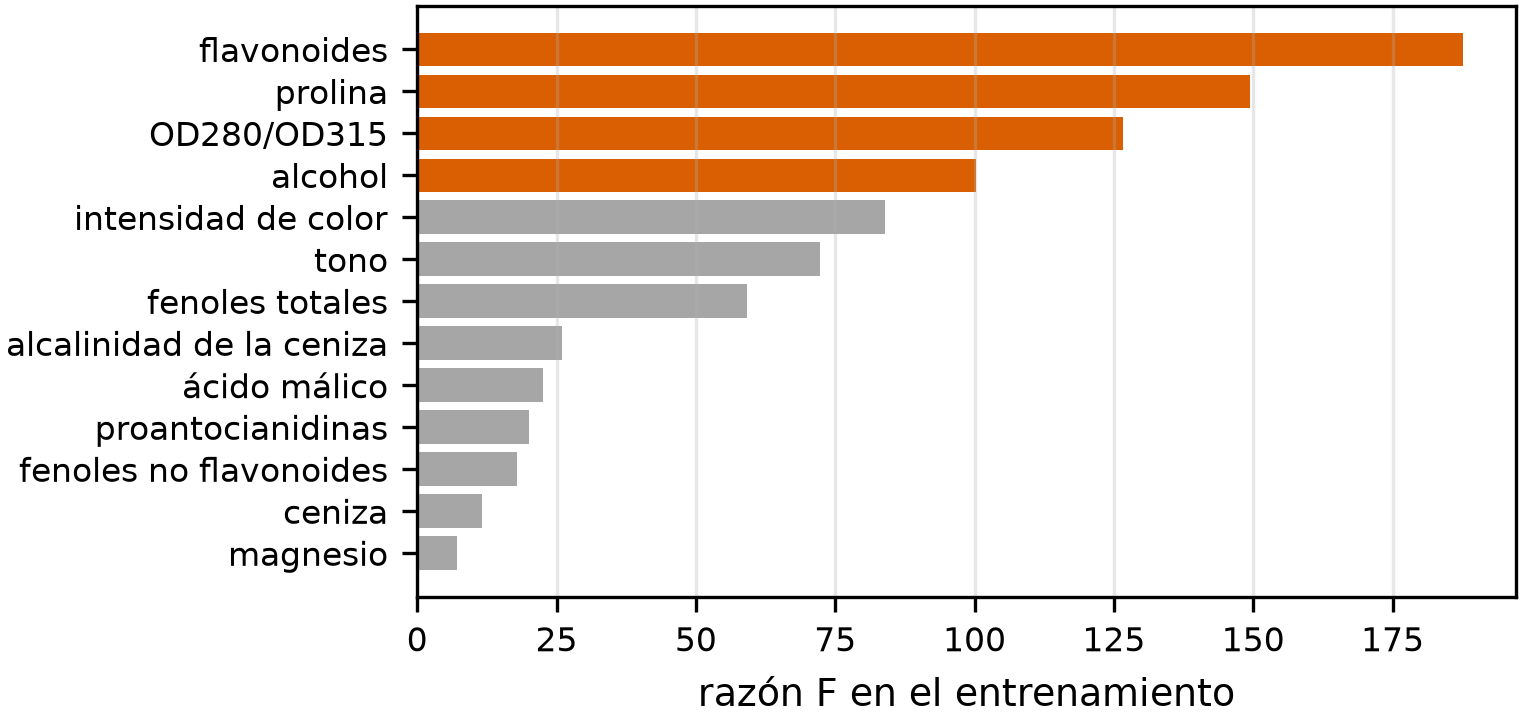
\includegraphics[width=11.5cm]{fig01_razon_f.png}
    \caption{Razón F de cada medida en el entrenamiento. En naranja las cuatro elegidas}
    \label{fig:f}
\end{figure}

\subsection{Función sigmoidal}

Las tres verificaciones de \texttt{sigmf} pasaron. El grado vale 0.5 en $x=c$, $\mathrm{sigmf}(5;[2\ 4]) = 1/(1+e^{-2}) = 0.8808$ y la función coincide con \texttt{skfuzzy.sigmf}, que recibe primero el centro y después la pendiente. La Figura~\ref{fig:mf} muestra la partición uniforme que usa el clasificador y tres sigmoidales con centro en 5.

\begin{figure}[!htb]
    \centering
    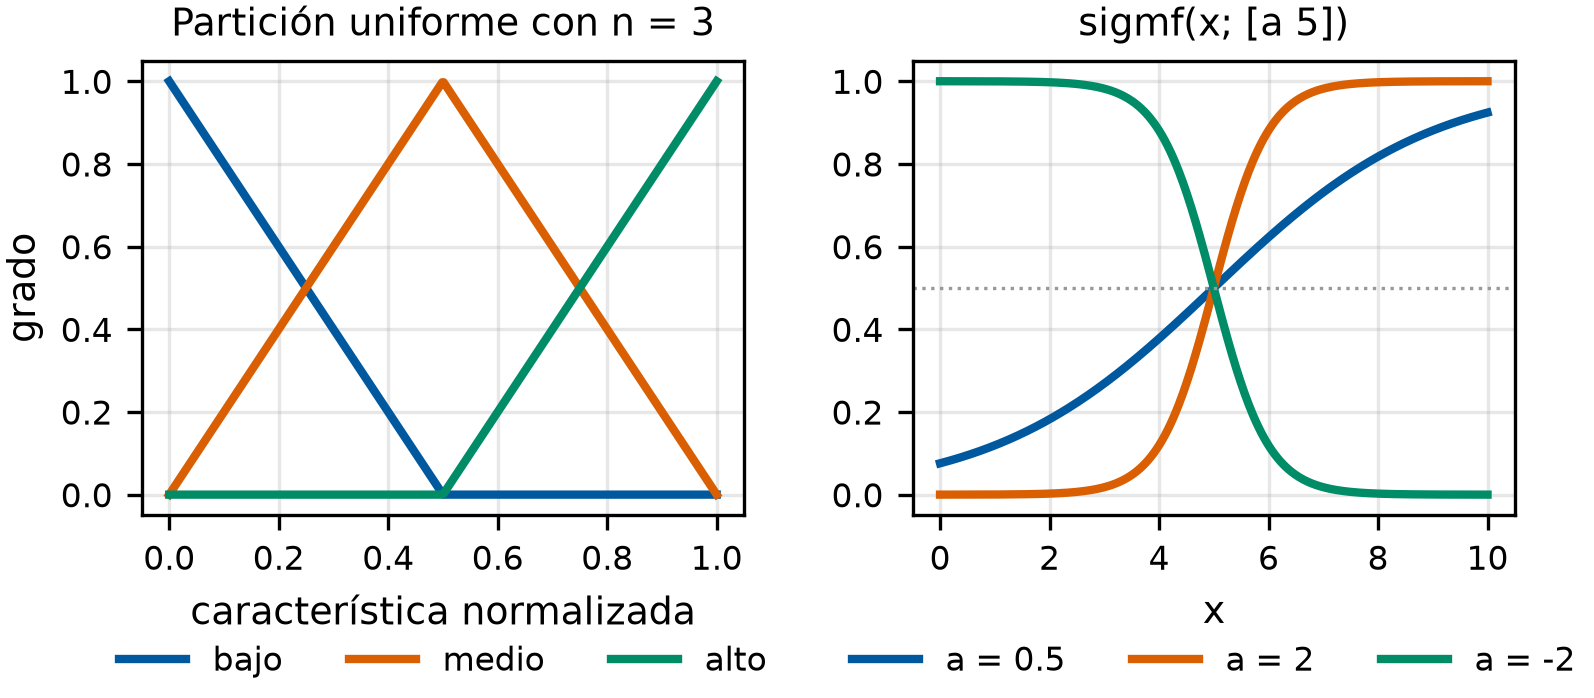
\includegraphics[width=14cm]{fig02_pertenencia.png}
    \caption{Izquierda, los tres triángulos de la partición uniforme. Derecha, \texttt{sigmf} con tres pendientes}
    \label{fig:mf}
\end{figure}

\subsection{Mínimo y producto}

Con $n=3$ el entrenamiento produjo \reglasTres{} reglas a partir de \nTr{} vinos. La exactitud en prueba fue \accProd~\% con el producto y \accMin~\% con el mínimo, y ninguna de las \nTe{} predicciones cambió al pasar de una t-norma a la otra. Como el mínimo es la mayor t-norma, la fuerza con el producto no puede superarla, y el punto de control lo confirma en el código. En \propiaTres{} de los \nTe{} vinos de prueba existe la regla formada por la etiqueta de mayor grado en cada medida, su celda propia, y en todos ellos esa regla es la ganadora. En los otros \otraTres{} gana una regla vecina. La regla de mayor grado se lee «si flavonoides es medio y prolina es medio y OD280/OD315 es medio y alcohol es medio entonces cultivar 2».

\subsection{Matriz de confusión}

La Figura~\ref{fig:cm3} muestra la matriz con $n=3$, la que pide la cuarta tarea. Hubo \erroresTres{} errores y el par más confundido fue \parReal{} tomado por \parPred{} (\parN{} veces). A los cuatro errores los decide su celda propia. En tres de ellos los vinos de entrenamiento de esa celda son de otro cultivar, 4 de 4, 15 de 16 y el único vino que cayó en ella. El cuarto cae en la celda de la regla de mayor grado de la sección anterior, que reúne 9 vinos del cultivar 1 y 7 del 2 y tomó la clase del vino de mayor grado, del cultivar 2. Es la única de las \reglasTres{} reglas cuyo consecuente no coincide con la mayoría de su celda. La fuerza de la regla ganadora en los errores fue de \fErrMin{} a \fErrMax, y en \nFErrAlta{} de ellos supera la mediana de los aciertos, \fOkMed.

\begin{figure}[!htb]
    \centering
    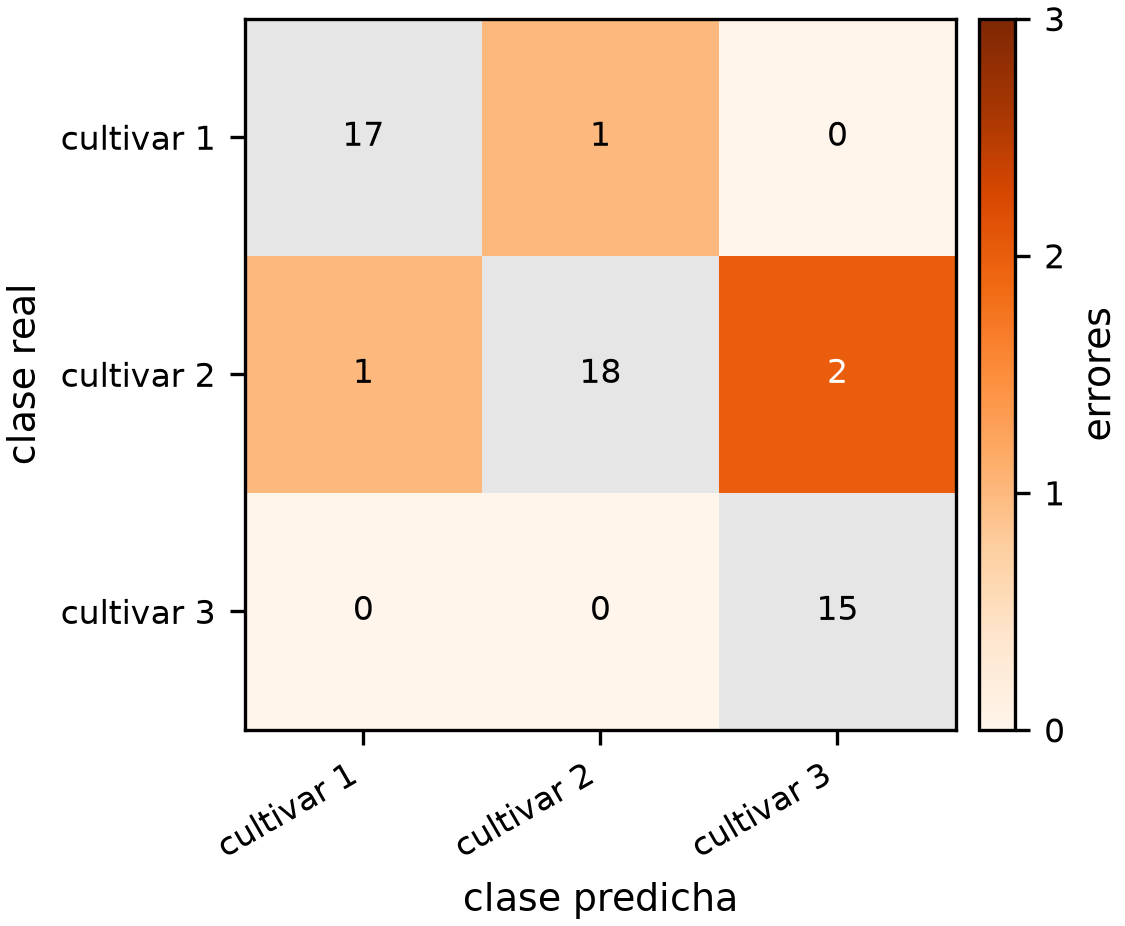
\includegraphics[width=7.2cm]{fig03_confusion_n3.png}
    \caption{Matriz de confusión en prueba con $n=3$. El color codifica solo los errores, con la misma escala que la Figura~\ref{fig:cm4}}
    \label{fig:cm3}
\end{figure}

\subsection{Etiquetas, reglas y exactitud}

La Tabla~\ref{tab:etiquetas} y la Figura~\ref{fig:etiquetas} reúnen la quinta tarea y la validación cruzada. El número de reglas crece con $n$ pero se queda lejos de la rejilla completa, porque solo aparecen las combinaciones que algún vino propone. El árbol no usa más de 13 hojas porque con ellas ya separa todo el entrenamiento, y logra \accArbol~\% en prueba con los cuatro límites probados. En validación cruzada obtiene \cvArbol~$\pm$~\cvArbolSd~\%.

\begin{table}[!htb]
    \centering
    \caption{Número de etiquetas, reglas y exactitud en porcentaje. La validación cruzada es la media y la desviación muestral de cinco particiones del entrenamiento}
    \label{tab:etiquetas}
    \footnotesize
    \begin{tabular}{c S[table-format=3.0] S[table-format=2.0] S[table-format=2.1] c S[table-format=2.1] S[table-format=2.0]}
        \toprule
        {\textbf{$n$}} & {\textbf{Rejilla $n^4$}} & {\textbf{Reglas}} & {\textbf{Prueba}} & \textbf{Validación cruzada} & {\textbf{Árbol, prueba}} & {\textbf{Hojas}} \\
        \midrule
\filasEtiquetas
        \bottomrule
    \end{tabular}
\end{table}

\begin{figure}[!htb]
    \centering
    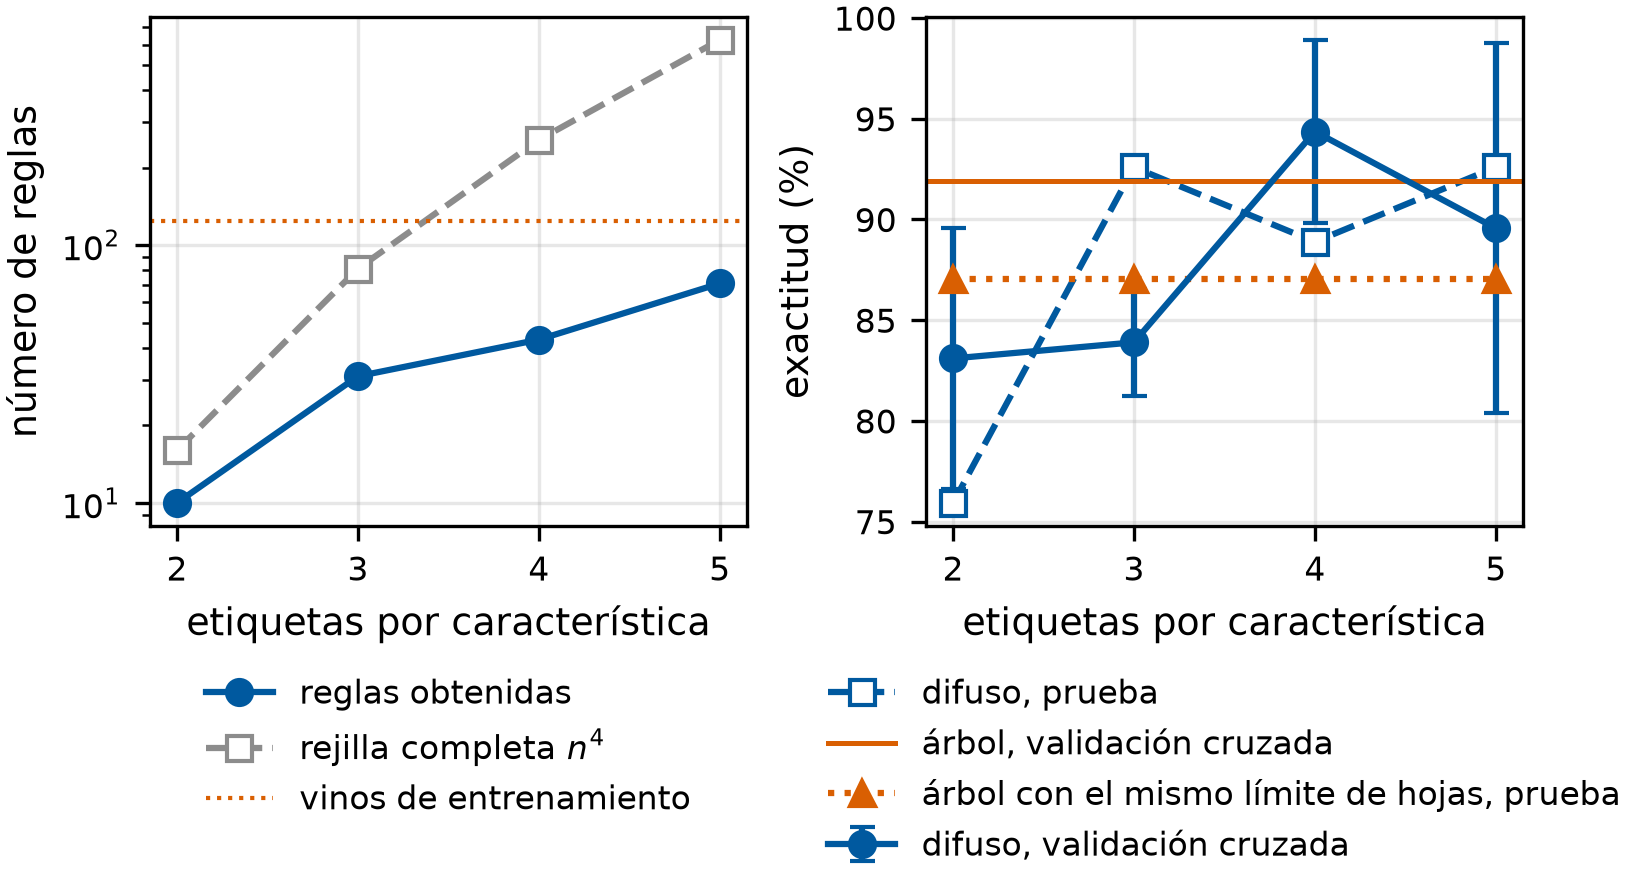
\includegraphics[width=15cm]{fig05_etiquetas.png}
    \caption{Izquierda, reglas obtenidas frente a la rejilla completa, en escala logarítmica. Derecha, exactitud del clasificador difuso y del árbol. Las barras son la desviación muestral de las cinco particiones}
    \label{fig:etiquetas}
\end{figure}

La validación cruzada favorece $n=\nElegido$ con \cvEleg~$\pm$~\cvElegSd~\%. Su error estándar es \eeEleg{} puntos y ningún $n$ menor queda a menos de esa distancia. En las 50 repeticiones con las semillas 0 a 49, $n=4$ tiene la mayor media en \repCuatro{} y $n=5$ en \repCinco. Las medias son \repMediaCuatro~\% para $n=4$, \repMediaTres~\% para $n=3$ y \repMediaArbol~\% para el árbol, y $n=4$ supera al árbol en las 50. El modelo elegido, con \reglasEleg{} reglas, obtiene \accEleg~\% en prueba, con un intervalo de Wilson del 95~\% entre \wilsonA{} y \wilsonB~\%. Sus \erroresEleg{} errores son todos vinos del cultivar 2, \errDosUno{} tomados por el cultivar 1 y \errDosTres{} por el 3, y el par más confundido empata (Figura~\ref{fig:cm4}). A cuatro los decide su celda propia, a uno una regla vecina porque su celda no está en la base, y uno no activa ninguna regla y recibe el cultivar 1, la clase por defecto. Las celdas que deciden esos errores tienen entre uno y tres vinos de entrenamiento. La Tabla~\ref{tab:origen} cuenta de dónde sale cada decisión según el número de etiquetas.

\begin{figure}[!htb]
    \centering
    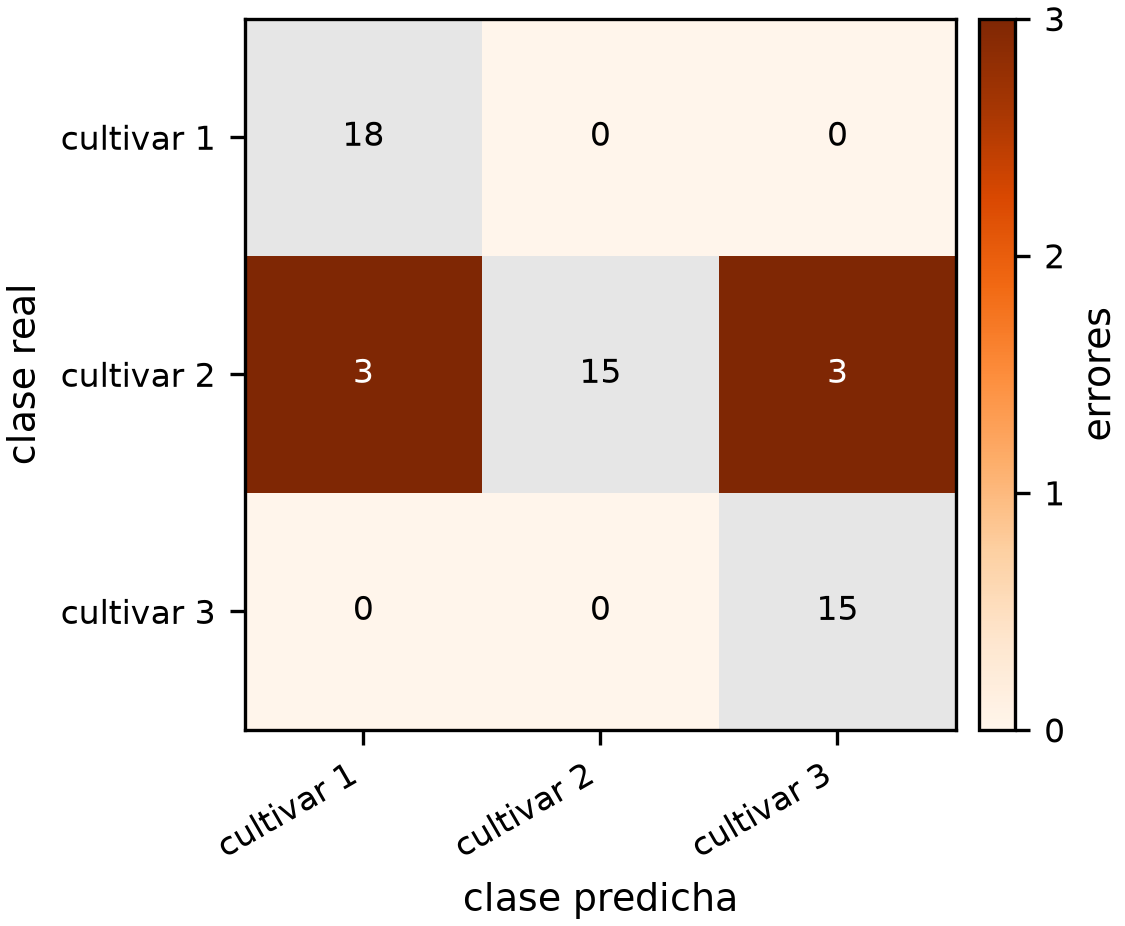
\includegraphics[width=7.2cm]{fig04_confusion_n4.png}
    \caption{Matriz de confusión en prueba con $n=\nElegido$, el número de etiquetas elegido por validación cruzada}
    \label{fig:cm4}
\end{figure}

\begin{table}[!htb]
    \centering
    \caption{Origen de las \nTe{} decisiones en prueba. La celda propia es la regla formada por la etiqueta de mayor grado en cada medida}
    \label{tab:origen}
    \footnotesize
    \begin{tabular}{c S[table-format=2.0] S[table-format=1.0] S[table-format=1.0]}
        \toprule
        {\textbf{$n$}} & {\textbf{Celda propia}} & {\textbf{Otra regla}} & {\textbf{Ninguna regla}} \\
        \midrule
\filasOrigen
        \bottomrule
    \end{tabular}
\end{table}

En prueba, el modelo elegido y el de $n=3$ discrepan en \the\numexpr\mcTresB+\mcTresC\relax{} vinos. Uno lo acierta solo el primero y \mcTresC{} solo el segundo, y la prueba de McNemar da $p=0.625$. Frente al árbol discrepan en \the\numexpr\mcArbB+\mcArbC\relax{} vinos, \mcArbB{} acertados solo por el modelo difuso y \mcArbC{} solo por el árbol, con $p=1$.

\subsection{Fuzzy C-Means y puente con MATLAB}

FCM convergió en \fcmIter{} iteraciones con $J=\fcmJ$. La Tabla~\ref{tab:fcm} compara sus grupos con los cultivares y la Figura~\ref{fig:fcm} los muestra sobre las dos medidas de mayor F. Al asignar cada vino al grupo de mayor grado, \fcmMal{} de los 178 quedan en un grupo dominado por otro cultivar, \fcmIntrusoN{} de ellos del \fcmIntruso{} en el grupo del \fcmDueno. De los \bajoN{} vinos cuyo grado máximo no llega a 0.6, \bajoDos{} son del cultivar 2, aunque ese cultivar es solo el \pctDos~\% de los vinos. El guion de MATLAB aplicó \texttt{fcm} con el mismo número de grupos, el mismo exponente y la misma escala. Su criterio de parada y su inicialización son los de MATLAB, pero obtuvo la misma partición, con un ARI de 1.000 frente a los grupos de Python y el mismo coeficiente de partición. Los centros coinciden a cuatro decimales salvo una coordenada, 0.7176 en Python y 0.7177 en MATLAB.

\begin{table}[!htb]
    \centering
    \caption{Agrupamiento de los 178 vinos con las cuatro medidas elegidas, sin usar el cultivar}
    \label{tab:fcm}
    \footnotesize
    \begin{tabular}{l S[table-format=1.3] S[table-format=1.3]}
        \toprule
        \textbf{Método} & {\textbf{ARI frente a los cultivares}} & {\textbf{Coeficiente de partición}} \\
        \midrule
        FCM en Python, $m=2$ & \ariFcm & \fpc \\
        \texttt{fcm} de MATLAB sobre los CSV exportados & 0.794 & 0.690 \\
        k-means & \ariKm & {--} \\
        \bottomrule
    \end{tabular}
\end{table}

\begin{figure}[!htb]
    \centering
    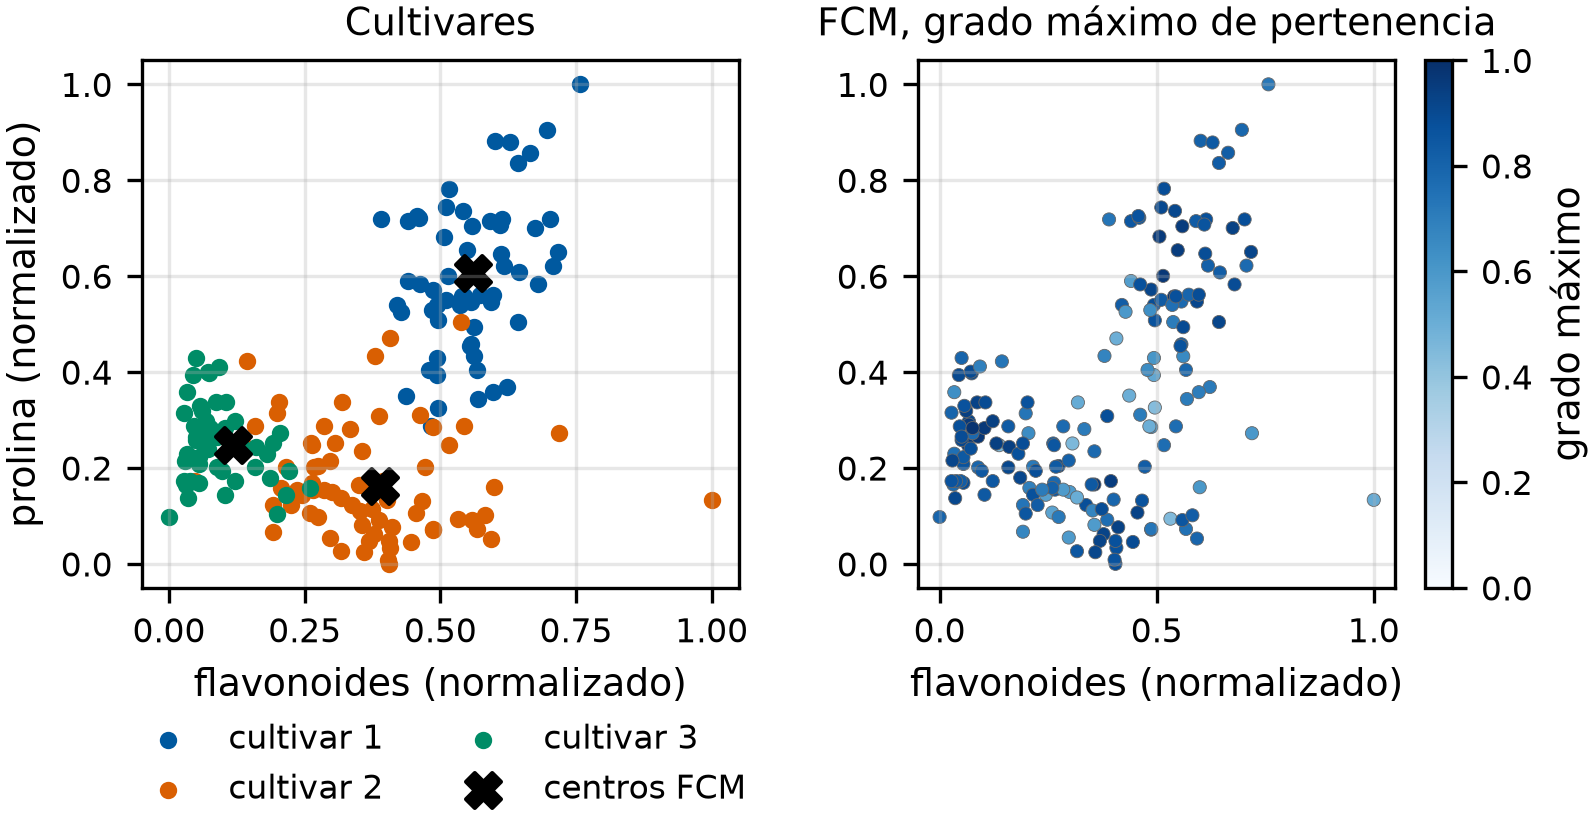
\includegraphics[width=15cm]{fig06_fcm.png}
    \caption{Izquierda, los cultivares y los centros de FCM. Derecha, el grado máximo de pertenencia de cada vino, más claro cuanto más compartido entre grupos}
    \label{fig:fcm}
\end{figure}

\subsection{Ajuste con ANFIS}

Las campanas iniciales de Python coinciden con las que imprime MATLAB para el sistema de \texttt{genfis}. Con los consecuentes en cero la salida es nula, así que el RMSE inicial, \rmseIni, es la raíz cuadrática media de la función que se aproxima y no dice nada de las campanas. La Tabla~\ref{tab:anfis} compara las diez épocas. Las diferencias con MATLAB llegan hasta \difRmse, los parámetros finales de las campanas difieren en menos de \difP{} y los de los consecuentes hasta en \difL. El tamaño de paso subió a 0.011 tras la quinta época y a 0.0121 tras la novena, como informa MATLAB. La Tabla~\ref{tab:campanas} muestra cómo se movieron las campanas y la Figura~\ref{fig:anfis} la aproximación.

\begin{table}[!htb]
    \centering
    \caption{RMSE de entrenamiento por época con ANFIS en Python y con \texttt{tunefis} en MATLAB R2026a, y tamaño de paso usado en cada época}
    \label{tab:anfis}
    \footnotesize
    \begin{tabular}{c S[table-format=1.7] S[table-format=1.7] c S[table-format=1.4]}
        \toprule
        \textbf{Época} & {\textbf{Python}} & {\textbf{MATLAB}} & \textbf{Diferencia absoluta} & {\textbf{Paso}} \\
        \midrule
\filasAnfis
        \bottomrule
    \end{tabular}
\end{table}

\begin{table}[!htb]
    \centering
    \caption{Parámetros $[a\ b\ c]$ de las cinco campanas antes y después de las diez épocas}
    \label{tab:campanas}
    \footnotesize
    \begin{tabular}{c S[table-format=1.4] S[table-format=1.4] S[table-format=2.4] S[table-format=1.4] S[table-format=1.4] S[table-format=2.4]}
        \toprule
         & \multicolumn{3}{c}{\textbf{Inicial (genfis)}} & \multicolumn{3}{c}{\textbf{Tras ANFIS}} \\
        \cmidrule(lr){2-4} \cmidrule(lr){5-7}
        \textbf{Campana} & {$a$} & {$b$} & {$c$} & {$a$} & {$b$} & {$c$} \\
        \midrule
\filasCampanas
        \bottomrule
    \end{tabular}
\end{table}

\begin{figure}[!htb]
    \centering
    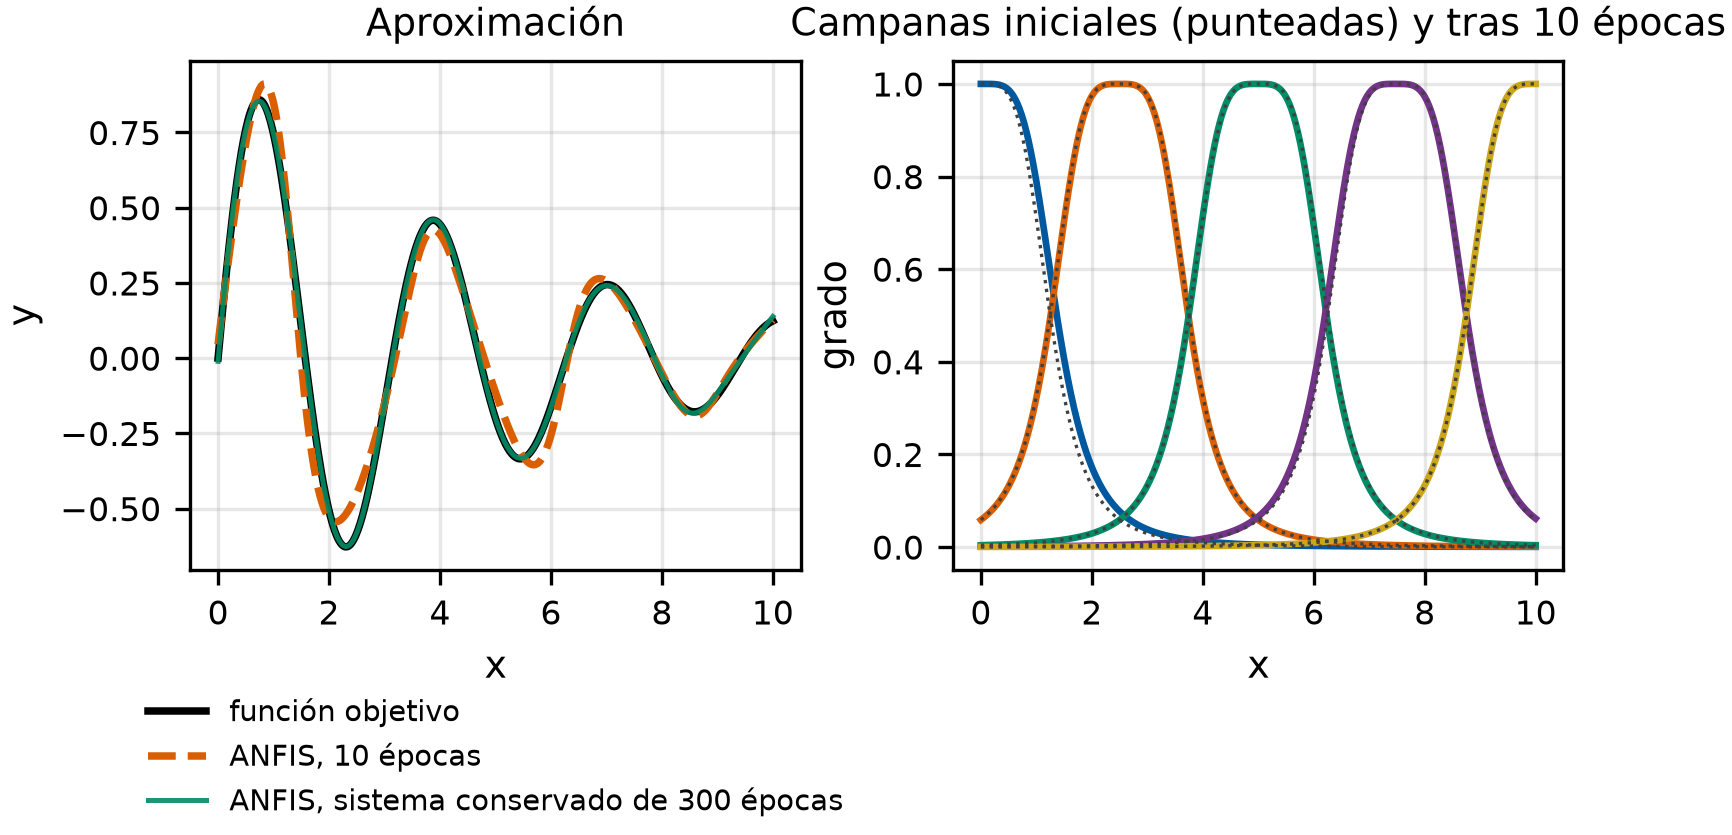
\includegraphics[width=15cm]{fig07_anfis.png}
    \caption{Izquierda, la función y las aproximaciones tras 10 épocas y del sistema conservado en 300 épocas. Derecha, las campanas iniciales y tras 10 épocas}
    \label{fig:anfis}
\end{figure}

En la ejecución de 300 épocas los primeros \cambiosIguales{} cambios del tamaño de paso coinciden con los de MATLAB, hasta la época \epIguales, y después las dos secuencias se separan. Python cambia el paso 69 veces y MATLAB 61, y el paso final es \pasoFin{} frente a 0.0020. El RMSE de entrenamiento en la época 300 es \rmseTres{} en Python y 0.00370 en MATLAB, y el de comprobación llega a su mínimo en la época \epMin{} en los dos, \valMin{} en Python y 0.00334 en MATLAB. En el sistema conservado los parámetros $a$ de las campanas quedan entre \aLargoMin{} y \aLargoMax{} y los centros se mueven hasta \cLargoMax. La Figura~\ref{fig:anfislargo} muestra las curvas de entrenamiento y de comprobación de Python.

\begin{figure}[!htb]
    \centering
    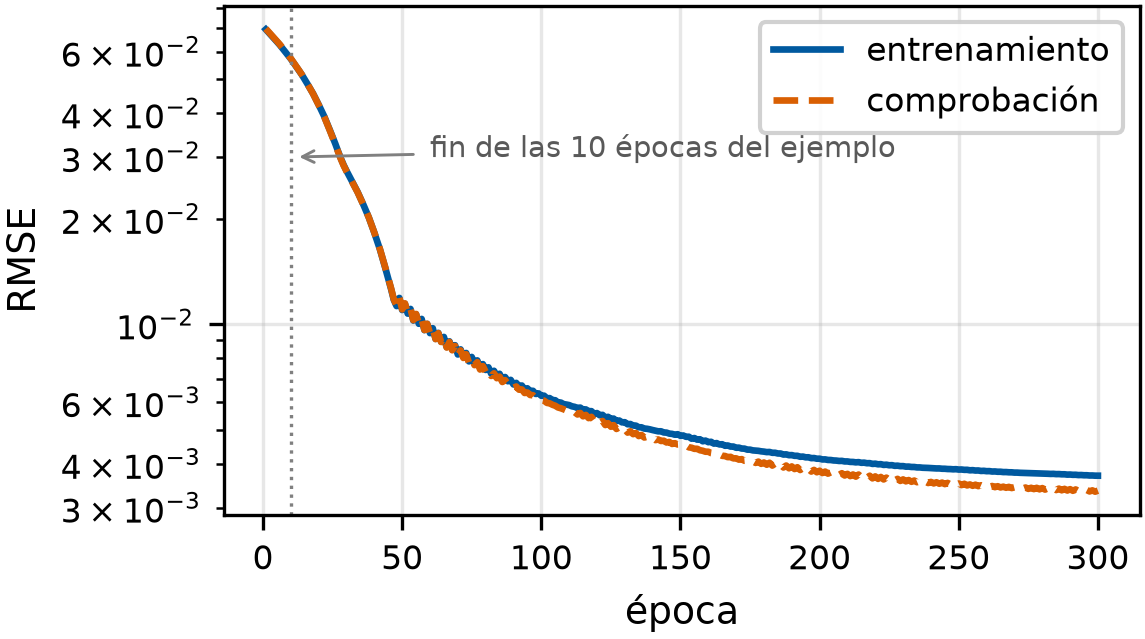
\includegraphics[width=8.5cm]{fig08_anfis_largo.png}
    \caption{RMSE de entrenamiento y de comprobación durante 300 épocas de ANFIS en Python}
    \label{fig:anfislargo}
\end{figure}

\section{Análisis}

\subsection{Las cuatro medidas elegidas}

La razón F elige las medidas que mejor separan los cultivares una por una, pero no mira si repiten información. Los flavonoides y la razón OD280/OD315 tienen una correlación de \corrAC, así que la tercera elegida repite en buena parte la información de la primera. Cuatro medidas bastan para que el clasificador difuso se quede alrededor del 90~\% con decenas de reglas, frente a las $3^{13}$ que tendría la rejilla con las 13 medidas y tres etiquetas. La elección, la normalización y la validación cruzada se hicieron dentro del entrenamiento para que la exactitud en prueba siga midiendo lo que el modelo hace con vinos nuevos.

\subsection{Por qué el mínimo y el producto coinciden}

La celda propia toma en cada medida la etiqueta de mayor grado, así que sus grados son, medida por medida, mayores o iguales que los de cualquier otra regla. Como toda t-norma es no decreciente en cada argumento, si esa celda está en la base gana o empata con el mínimo, con el producto y con cualquier otra t-norma. Con $n=3$ está en la base para \propiaTres{} de los \nTe{} vinos de prueba. En esos vinos la coincidencia es una propiedad del clasificador, y solo los otros \otraTres{} dependían de los datos, que tampoco cambiaron de clase. En general el producto se aparta del mínimo cuando hay varios grados intermedios. Con los grados (0.6, 0.6, 0.6, 0.6) el mínimo da 0.6 y el producto 0.13, mientras que con (0.5, 1, 1, 1) los dos dan 0.5. La Tabla~\ref{tab:origen} muestra que la propiedad pierde alcance cuando crecen las etiquetas, porque cada vez más vinos tienen su celda propia fuera de la base y deciden por otra regla o por la clase por defecto.

\subsection{De dónde salen los errores}

Todos los errores, con $n=3$ y con el modelo elegido, involucran al cultivar 2. En la Figura~\ref{fig:fcm} ese cultivar tiene flavonoides intermedios entre los del 1 y los del 3 y la prolina más baja de los tres, y comparte parte de esa zona con cada vecino. Con $n=3$, tres de los cuatro errores caen en celdas cuyos vinos de entrenamiento son, todos o casi todos, de otro cultivar. Con estas cuatro medidas y tres etiquetas esos vinos están en la zona de su vecino, y cambiar el consecuente por la mayoría no los corregiría. Solo un error viene del consecuente, el de la celda con 9 vinos del cultivar 1 y 7 del 2, porque Wang y Mendel toma la clase del vino de mayor grado y no de la mayoría. Con más etiquetas las celdas se vacían. Con $n=4$ las que deciden los errores tienen entre uno y tres vinos de entrenamiento, y un vino no activa ninguna regla y recibe la clase por defecto. Con $n=5$ son dos los vinos sin regla. Una fuerza nula delata al vino sin regla, pero en los demás errores la fuerza no avisa. Mide qué tan cerca está el vino del punto de la rejilla donde todas las etiquetas de la regla valen 1, que no tiene que ver con la fiabilidad del consecuente, y dos de los cuatro errores con $n=3$ tienen una fuerza mayor que la mediana de los aciertos.

\subsection{Etiquetas, reglas e interpretabilidad}

Con dos etiquetas las reglas son pocas y se leen bien, pero el clasificador pierde exactitud. De tres a cinco etiquetas las reglas pasan de \reglasTres{} a más de setenta para \nTr{} vinos, más de una regla por cada dos vinos, y la exactitud en prueba no sube de forma sostenida. La validación cruzada y la prueba no coinciden en el mejor $n$. La primera prefiere 4, que tiene la mayor media en \repCuatro{} de 50 repeticiones, mientras que en prueba $n=3$ acierta dos vinos más. La prueba de McNemar no distingue esos dos modelos, ni el elegido del árbol, y el intervalo de Wilson del modelo elegido mide cerca de 17 puntos de ancho. Con \nTe{} vinos de prueba ninguna de esas diferencias es concluyente, y el modelo que se reporta es el elegido sin mirar la prueba. En validación el difuso con $n=4$ supera al árbol en las 50 repeticiones, \repMediaCuatro{} frente a \repMediaArbol~\% en promedio, pero todas reparten los mismos \nTr{} vinos y la prueba, con \nTe, no alcanza para confirmarlo.

\subsection{Agrupamiento con FCM}

FCM recupera los cultivares casi igual que k-means, con un ARI de \ariFcm{} frente a \ariKm. Además entrega el grado de cada vino en cada grupo. El cultivar 2 es el \pctDos~\% de los vinos, pero reúne \bajoDos{} de los \bajoN{} vinos con grado máximo menor que 0.6, el mismo cultivar en el que se equivoca el clasificador supervisado. El coeficiente de partición de \fpc{} queda entre $1/3$ y 1, una partición con grupos reconocibles pero con frontera compartida. MATLAB obtiene la misma partición con otra inicialización y otro criterio de parada, así que el resultado no depende de la implementación.

\subsection{Ajuste con ANFIS}

En las diez épocas del ejemplo el sistema de Python sigue al de MATLAB época por época. Las diferencias en el RMSE son del orden del redondeo de los siete decimales que imprime MATLAB. Las de los consecuentes, de hasta \difL, son compatibles con que MATLAB estime los mínimos cuadrados de forma secuencial, como propone Jang (1993), mientras que Python los resuelve de forma directa. La primera época, en la que las campanas son todavía las iniciales y solo se ajustan los consecuentes, deja el RMSE en \rmseUno, y las nueve siguientes solo lo bajan a \rmseFin. Las campanas apenas se mueven, la de la izquierda se corre 0.056 y las demás menos.

En 300 épocas la secuencia de pasos de Python se separa de la de MATLAB después de la época \epIguales, señal de que la regla programada difiere en algún detalle de la de MATLAB. Aun así el error final coincide, al menos en este ejemplo. Como la función no tiene ruido, la curva de comprobación solo muestra que el sistema interpola bien entre los puntos de entrenamiento. Además el sistema conservado se elige con el error de comprobación, y por eso su mínimo de \valMin{} no es una estimación independiente del error.

\section{Conclusiones}

Las seis tareas del taller propuesto quedaron resueltas en Python sobre las funciones del cuaderno resuelto, con las veintiuna verificaciones del cuaderno en \texttt{[OK]}.

Con cuatro medidas elegidas por razón F en el entrenamiento y cuatro etiquetas elegidas por validación cruzada, el clasificador con reglas extraídas de Wine obtiene \accEleg~\% en prueba con \reglasEleg{} reglas. Con tres etiquetas obtuvo \accNtres~\% en prueba, pero la validación estima \cvTres~\% para esa configuración, y McNemar no distingue los dos modelos con \nTe{} vinos.

El mínimo y el producto dan las mismas predicciones porque la celda propia de cada vino gana con cualquier t-norma cuando existe. Todos los errores involucran al cultivar 2. Con tres etiquetas, tres de los cuatro caen en celdas cuyos vinos de entrenamiento son de otro cultivar y el cuarto en la única regla cuyo consecuente no sigue a la mayoría. Con más etiquetas los errores salen de celdas con uno a tres vinos y se suman vinos que no activan ninguna regla.

FCM recupera los cultivares con un ARI de \ariFcm, casi igual que k-means (\ariKm), y \texttt{fcm} de MATLAB sobre los CSV exportados produce la misma partición.

El algoritmo ANFIS programado en Python reproduce el ejemplo de \texttt{tunefis} de MathWorks durante las diez épocas, con diferencias de hasta \difRmse{} en el RMSE. Diez épocas mejoran sobre todo los consecuentes. Con 300 el error baja unas \reduccion{} veces y termina en el mismo valor que MATLAB, aunque la secuencia de pasos se separa después de la época \epIguales.

\section{Referencias}
\begin{itemize}
    \item Aeberhard, S., Coomans, D., \& de Vel, O. (1994). Comparative analysis of statistical pattern recognition methods in high dimensional settings. \textit{Pattern Recognition}, 27(8), 1065--1077.
    \item Bezdek, J. C., Ehrlich, R., \& Full, W. (1984). FCM: The fuzzy c-means clustering algorithm. \textit{Computers \& Geosciences}, 10(2--3), 191--203.
    \item Hubert, L., \& Arabie, P. (1985). Comparing partitions. \textit{Journal of Classification}, 2(1), 193--218.
    \item Jang, J.-S. R. (1993). ANFIS: Adaptive-network-based fuzzy inference system. \textit{IEEE Transactions on Systems, Man, and Cybernetics}, 23(3), 665--685.
    \item MathWorks (2026). \textit{Fuzzy Logic Toolbox. tunefis y el ejemplo Tune Fuzzy Inference System}. Documentación de MATLAB R2026a.
    \item McNemar, Q. (1947). Note on the sampling error of the difference between correlated proportions or percentages. \textit{Psychometrika}, 12(2), 153--157.
    \item Takagi, T., \& Sugeno, M. (1985). Fuzzy identification of systems and its applications to modeling and control. \textit{IEEE Transactions on Systems, Man, and Cybernetics}, 15(1), 116--132.
    \item Wang, L.-X., \& Mendel, J. M. (1992). Generating fuzzy rules by learning from examples. \textit{IEEE Transactions on Systems, Man, and Cybernetics}, 22(6), 1414--1427.
    \item Zadeh, L. A. (1965). Fuzzy sets. \textit{Information and Control}, 8(3), 338--353.
\end{itemize}

\clearpage
\appendix
\section{Código de los bloques completados}
\label{anexo:codigo}

Se reproducen los seis bloques \texttt{TODO} tal como quedaron en el cuaderno entregado.

\begin{lstlisting}[caption={TODO 1, cuatro características con el entrenamiento}]
def elegir_caracteristicas(X, y, k=4):
    F, _ = f_classif(X, y)
    return np.argsort(-F)[:k], F

idx, F_tr = elegir_caracteristicas(d["Xtr"], d["ytr"])
\end{lstlisting}

\begin{lstlisting}[caption={TODO 2, función sigmoidal}]
def sigmf(x, a, c):
    """Sigmoidal [a c]: 1 / (1 + exp(-a (x - c)))."""
    x = np.asarray(x, dtype=float)
    return 1.0 / (1.0 + np.exp(-a * (x - c)))
\end{lstlisting}

\begin{lstlisting}[caption={TODO 3, fuerza de las reglas con mínimo o producto}]
def fuerza_reglas(G, R, tnorma="prod"):
    """G: N x F x n_mf grados de pertenencia. R: n_reglas x F etiquetas. Devuelve N x n_reglas."""
    grados = G[:, np.arange(G.shape[1])[None, :], R]          # N x n_reglas x F
    return grados.min(axis=2) if tnorma == "min" else grados.prod(axis=2)
\end{lstlisting}

\begin{lstlisting}[caption={TODO 4, matriz de confusión y par más confundido}]
cm = confusion_matrix(d["yte"], pred_prod)
fuera = cm.copy(); np.fill_diagonal(fuera, 0)
par = tuple(int(v) for v in np.unravel_index(np.argmax(fuera), fuera.shape))
\end{lstlisting}

\begin{lstlisting}[caption={TODO 5, etiquetas, reglas, exactitud y árbol}]
filas = []
for n in (2, 3, 4, 5):
    Rn, cn, gn = extraer_reglas(Xtr, d["ytr"], n)
    pn, _ = predecir_tnorma(Xte, Rn, cn, n)
    arbol = DecisionTreeClassifier(max_leaf_nodes=max(2, len(Rn)), random_state=SEMILLA)
    arbol.fit(d["Xtr"][:, idx], d["ytr"])
    pa = arbol.predict(d["Xte"][:, idx])
    filas.append((n, len(Rn), accuracy_score(d["yte"], pn), accuracy_score(d["yte"], pa), int(arbol.get_n_leaves())))
\end{lstlisting}

\begin{lstlisting}[caption={TODO 6, FCM y exportación para MATLAB}]
X_all = np.vstack([d["Xtr"], d["Xte"]])[:, idx]; y_all = np.concatenate([d["ytr"], d["yte"]])
Xa = normalizar(X_all, X_all.min(0), X_all.max(0))
centros, U, J = fcm_propio(Xa, c=3, m=2.0)
for nombre, X_, y_ in (("train", d["Xtr"], d["ytr"]), ("test", d["Xte"], d["yte"])):
    tabla = pd.DataFrame(X_[:, idx], columns=car4)
    tabla["clase"] = y_ + 1                                   # MATLAB numera desde 1
    tabla.to_csv(f"wine_4car_{nombre}.csv", index=False)
pd.DataFrame({"grupo_python": U.argmax(axis=0) + 1}).to_csv("wine_fcm_python.csv", index=False)
\end{lstlisting}

\section{Salida de los guiones de MATLAB}
\label{anexo:matlab}

Salida de \texttt{referencia\_tunefis\_matlab.m} en MATLAB R2026a, sin las líneas en blanco, la descripción de la red ni los avisos de inicio y fin del entrenamiento que imprime \texttt{tunefis}.

\begin{lstlisting}[language={}, numbers=none, caption={Salida de referencia\_tunefis\_matlab.m}]
campana inicial 1  gbellmf [1.250000 2.000000 0.000000]
campana inicial 2  gbellmf [1.250000 2.000000 2.500000]
campana inicial 3  gbellmf [1.250000 2.000000 5.000000]
campana inicial 4  gbellmf [1.250000 2.000000 7.500000]
campana inicial 5  gbellmf [1.250000  2.000000 10.000000]
RMSE inicial 0.3466485
1    0.0694086
2    0.0680259
3    0.066663
4    0.0653198
Step size increases to 0.011000 after epoch 5.
5    0.0639961
6    0.0626917
7    0.0612787
8    0.0598881
Step size increases to 0.012100 after epoch 9.
9    0.0585193
10   0.0571712
Minimal training RMSE = 0.0571712
RMSE final 0.0571712
campana final 1  [1.313552 1.999443 0.056200]
campana final 2  [1.241396 1.985618 2.498113]
campana final 3  [1.242335 1.998512 4.988612]
campana final 4  [1.275471 1.999512 7.477887]
campana final 5  [1.251139 1.999575 9.999436]
consecuente final 1  [1.872801 0.215714]
consecuente final 2  [0.848484 -3.096972]
consecuente final 3  [-0.639171  2.859215]
consecuente final 4  [-0.487932  3.894183]
consecuente final 5  [0.123148 -1.032788]
300 épocas. RMSE de entrenamiento en la época 10 0.05717 y en la 300 0.00370
300 épocas. RMSE de comprobación mínimo 0.00334 en la época 299
300 épocas. Paso final 0.0020
Épocas en que cambia el paso: 6 10 14 18 22 26 30 34 38 42 46 53 57 61 65 69 73 77 81 85 89 93 97 101 108 114 119 123 127 131 135 139 142 148 153 159 166 171 177 183 190 195 201 207 214 219 225 232 237 243 249 256 262 267 271 275 279 283 286 292 298
\end{lstlisting}

\begin{lstlisting}[language={}, numbers=none, caption={Salida de puente\_matlab\_wine.m}]
Vinos: 178 | coeficiente de partición: 0.690
ARI frente a los cultivares: 0.794
ARI frente a los grupos del FCM de Python: 1.000
Centros ordenados por la primera característica:
    0.1179    0.2474    0.1724    0.5343
    0.3883    0.1626    0.6146    0.3151
    0.5605    0.6061    0.6884    0.7177
Grupo frente a cultivar:
    57     1     0
     2    60     0
     0    10    48
\end{lstlisting}

\end{document}
